\chapter{Synchronous and Asynchronous Communication Mechanisms}\label{ch:sync-async-communication}

\section{Overview of Synchronous and Asynchronous Communication}\label{sec:5-sync-async-overview}

\subsection{Overview of Synchronous Communication}\label{subsec:5-sync-communication-overview}

The synchronous (Synchronous) communication mechanism in an operating system is a mechanism used to synchronize two parallel or concurrent processes. In traditional operating systems it usually manifests as mechanisms such as pipes and semaphores. The greatest characteristic of the synchronous communication mechanism is its blocking nature, that is, after one side sends, if the other side does not receive, the sender blocks, and the sender's blocking is only released after the receiver receives. If the receiver receives first, then it also blocks, and the receiver's blocking is only released after the sender sends. Synchronous communication using this traditional implementation requires two threads in order to communicate between processes.

In RME, the synchronous communication model is further simplified into the thread migration (Thread
Migration) invocation\footnote{or a local procedure call}, which allows a thread to enter another process, execute a piece of code inside it, and then return to its own process to continue execution. This is one of the most efficient inter-process communication (Inter-Process
Communication, IPC) implementations. Because this kind of invocation allows one execution flow to cross process boundaries, it can only be used when the two processes trust each other to a considerable degree. Its apparent result is as if a thread running inside one process directly invoked a function inside another process, so that only one thread is needed to perform inter-process communication. If this synchronous invocation is to use extra parameters, then these parameters are passed through shared memory, register sets, or coprocessor register sets. Synchronous invocations can be nested, and the number of nesting levels can be unlimited. An example of thread migration is shown below. This thread performs two migrations and alternately executes among three processes. In the figure, the red upright triangles represent invocation activation, and the red inverted triangles represent invocation return. In process 2 and process 3, the boxes on the thread's execution flow mark the thread's invocation stack, and the black triangle points to the top of the invocation stack. When returning, control always first returns into the process indicated by the top of the stack.

\begin{figure}[htbp]
    \centering
    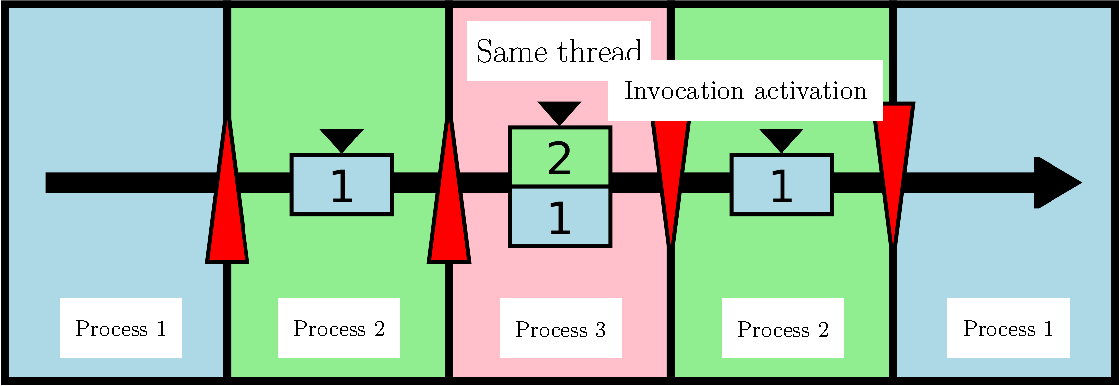
\includegraphics[width=0.72\textwidth]{Figure/image12.pdf}
    \caption{Example of Synchronous Thread Migration}
    \label{fig:5-1-sync-thread-migration-example}
\end{figure}

The design of the synchronous invocation refers to Composite\hyperref[cite:5-1]{{[}1{]}} and Mach 3\hyperref[cite:5-2]{{[}2{]}}.

\subsection{Overview of Asynchronous Communication}\label{subsec:5-async-communication-overview}

The asynchronous (Asynchronous) communication mechanism in an operating system is used to coordinate the producer-consumer (Producer-Consumer) problem in the operating system. Generally, such mechanisms include the mailbox (Mailbox), the message queue (Message
Queue), and so on. The greatest characteristic of the asynchronous communication mechanism is its non-blocking nature, that is, after one side issues, if the other side does not receive, the information is first buffered, and then the sender returns directly. When receiving, if there is information, the receiver returns; if there is no information, then depending on the system call, the receiver may return directly, may block, or may block for a period of time until a timeout and then return.

In RME, the asynchronous communication model is further simplified into the signal endpoint (Signal
Endpoint), whose main mechanism is to enable the sender to send to the signal endpoint and the receiver to receive from the signal endpoint. Sending is always non-blocking, receiving is also non-blocking when there is a signal, and receiving when there is no signal may either block or not block. A signal only carries quantity information\footnote{it has only one counter}, and does not carry any other information. If other information needs to be transferred, then the transfer of this information needs to be accomplished in user mode through shared memory (Shared
Memory). An example of asynchronous communication is shown below. In it, thread 1, which has a lower priority, sends an asynchronous signal (red lightning bolt symbol) to thread 2, which has a higher priority; after thread 2 finishes processing, it blocks on the endpoint again (red rectangle symbol), so that thread 1 continues execution.

\begin{figure}[htbp]
    \centering
    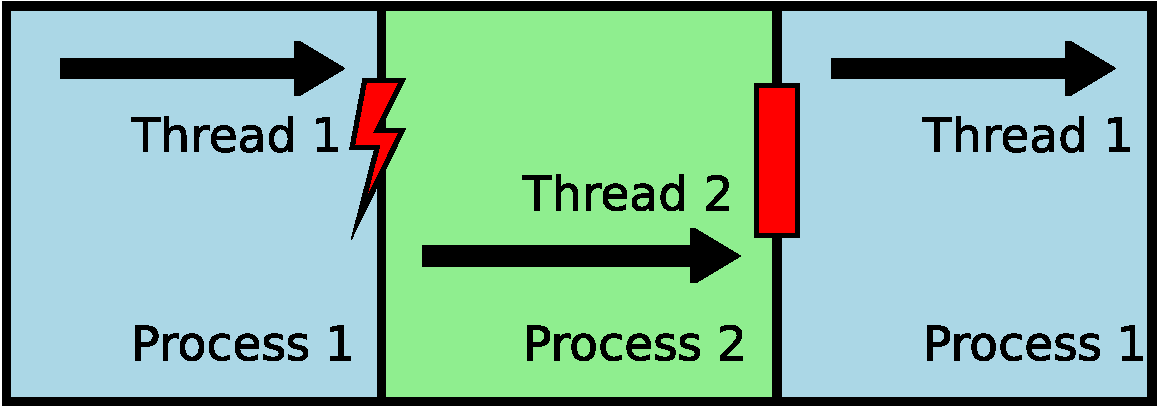
\includegraphics[width=0.72\textwidth]{Figure/image13.pdf}
    \caption{Example of Asynchronous Signal Sending and Receiving}
    \label{fig:5-2-async-signal-send-receive-example}
\end{figure}

\section{Synchronous Communication Operations}\label{sec:5-sync-communication-operations}

To use the synchronous communication functionality, one must first create a synchronous invocation. When creating a synchronous invocation, the process needs to be specified. After creation, the entry of the invocation inside this process and the stack to be used by the thread need to be specified. Next, the synchronous invocation is performed, and the thread transitions from inside one thread to execute inside another process. If other synchronous invocations are used within this synchronous invocation, then the synchronous invocations will nest (Nesting). After the synchronous invocation finishes execution, the synchronous invocation return function needs to be called to return from this synchronous invocation. Compared with asynchronous communication, synchronous communication operations have immediacy, guaranteeing that a response will definitely be obtained at the fastest possible speed when the invocation is made, and when the invocation is made the thread merely crosses into another protection domain to execute without changing its other attributes. Note that the synchronous invocation does not save any general-purpose registers or coprocessor registers, nor does it change the coprocessor's current state; it only changes those registers necessary for changing the program's execution flow, such as the stack pointer and the program counter. The values of the general-purpose registers and the coprocessor state will be carried directly to the thread migration entry and exit. If there are registers or coprocessor states that need to be saved, then user mode needs to do so itself. In addition, the coprocessor register set can also be used to pass extra parameters or receive extra return values.

A synchronous invocation is not bound to a CPU. If threads on multiple CPUs attempt to activate one synchronous invocation at the same time, then only the thread on one CPU will succeed, and the other threads will all return error codes; if an attempt is made to activate a synchronous invocation again while it is already activated\footnote{regardless of whether on the same CPU or on a different CPU}, then an error code will also be returned.

If nesting occurs within synchronous invocations, then returning also needs to be done level by level. If the thread is unbound while performing a synchronous invocation, then it remains in the invocation state, and after being bound to a new CPU it will continue executing from there; if an error occurs while the thread is performing a synchronous invocation, the thread's behavior is determined by the Fault\_Ret\_Flag parameter passed in when setting the invocation execution properties. If this parameter is not 0, then it does not enter the RME\_THD\_EXCPEND state, but instead returns directly from this synchronous invocation to the previous level, and the return value is an error code indicating that an error occurred. If this parameter is 0, then the thread enters the RME\_THD\_EXCPEND state and waits for the error to be repaired.

\section{Asynchronous Communication Operations}\label{sec:5-async-communication-operations}

To use the asynchronous communication functionality, one must first create a signal endpoint, then have the sender send a signal to it, and the receiver receives from this endpoint. When receiving, if the endpoint has no signal, then the receiver blocks; if the reception succeeds, then the return value will be the number of remaining signals at the time of the successful return.

A signal endpoint is not bound to a CPU. If threads on multiple CPUs simultaneously attempt to block on one endpoint, then only one will succeed, and the other threads will all return an error value. If, when a thread has already blocked on an endpoint, other threads also attempt to block\footnote{regardless of whether on the same CPU or on a different CPU}, then the blocking of the other threads will fail. In practice, the usage of one signal endpoint with multiple receivers is not recommended, because this often requires fairly complex coordination.

Note that when a thread has already blocked on a signal endpoint, only a send operation on the same CPU as the blocked thread can release that thread's blocking. Although threads on other CPUs can also send to that endpoint, they can only increase the signal count and cannot release the blocking.

RME does not allow the initial (Init) thread to receive any signals. Because receiving a signal is a potentially blocking operation, and once the Init thread blocks, RME cannot guarantee that it will be able to find a thread to run when the CPU is idle. If it is necessary both to receive signals and for the receiving thread's timeslice to be infinite, then one can create a new thread and then perform an infinite transfer from Init to it, turning it into an infinite thread.

\needspace{16\baselineskip}
In order to make application programming more flexible, RME permits four different methods of receiving endpoint signals, which are as follows:

\begin{xltabular}{\textwidth}{@{}>{\hsize=0.5583\hsize\raggedright\arraybackslash}X>{\hsize=1.4417\hsize\raggedright\arraybackslash}X@{}}
\caption{Four Receiving Options of Endpoint Signals}\label{tab:5-1-endpoint-signal-receive-methods}\\
\toprule
Receiving Option & Meaning\tabularnewline
\endfirsthead
\toprule
Receiving Option & Meaning\tabularnewline
\midrule
\endhead
\bottomrule
\endlastfoot
RME\_RCV\_BS &
Attempt to receive a single signal in a blocking manner. May cause the thread itself to block.\tabularnewline
RME\_RCV\_BM &
Attempt to receive multiple signals in a blocking manner. May cause the thread itself to block, and if there are signals on the endpoint, all signals on the endpoint will be obtained.\tabularnewline
RME\_RCV\_NS &
Attempt to receive a single signal in a non-blocking manner. This method returns immediately when there is no signal on the endpoint.\tabularnewline
RME\_RCV\_NM &
Attempt to receive multiple signals in a non-blocking manner. This method returns immediately when there is no signal on the endpoint, and if there are signals on the endpoint, all signals on the endpoint will be obtained.\tabularnewline
\end{xltabular}
\nopagebreak[4]

\section{List of Synchronous Communication Functions}\label{sec:5-sync-communication-function-list}

The kernel functions related to synchronous invocations are as follows:

\begin{xltabular}{\textwidth}{@{}>{\hsize=0.8854\hsize\raggedright\arraybackslash}X>{\hsize=0.6747\hsize\raggedright\arraybackslash}X>{\hsize=1.4400\hsize\raggedright\arraybackslash}X@{}}
\caption{Kernel Functions Related to Synchronous Communication}\label{tab:5-2-sync-communication-kernel-functions}\\
\toprule
Call number & Type & Purpose\tabularnewline
\endfirsthead
\toprule
Call number & Type & Purpose\tabularnewline
\midrule
\endhead
\bottomrule
\endlastfoot
RME\_SVC\_INV\_CRT & System call & Create a synchronous invocation\tabularnewline
RME\_SVC\_INV\_DEL & System call & Delete a synchronous invocation\tabularnewline
RME\_SVC\_INV\_SET & System call &
Set the execution properties of the synchronous invocation\footnote{entry and stack}\tabularnewline
RME\_SVC\_INV\_ACT & System call &
Activate\footnote{perform or invoke} a synchronous invocation\tabularnewline
RME\_SVC\_INV\_RET & System call & Return from a synchronous invocation\tabularnewline
\end{xltabular}
\nopagebreak[4]

The operation flags of the synchronous invocation capability are as follows:

\begin{xltabular}{\textwidth}{@{}>{\hsize=0.9420\hsize\raggedright\arraybackslash}X>{\hsize=0.6957\hsize\raggedright\arraybackslash}X>{\hsize=1.3622\hsize\raggedright\arraybackslash}X@{}}
\caption{Synchronous Invocation Operation Flags}\label{tab:5-3-sync-invocation-operation-flags}\\
\toprule
Flag & Bit & Purpose\tabularnewline
\endfirsthead
\toprule
Flag & Bit & Purpose\tabularnewline
\midrule
\endhead
\bottomrule
\endlastfoot
RME\_INV\_FLAG\_SET & {[}0{]} &
Allow setting the execution properties of this synchronous invocation.\tabularnewline
RME\_INV\_FLAG\_ACT & {[}1{]} & Allow activating this synchronous invocation.\tabularnewline
\end{xltabular}
\nopagebreak[4]

Since the synchronous invocation return operation does not require the synchronous invocation capability, there is no such operation flag bit either\footnote{see Section~\ref{subsec:5-return-from-sync-invocation} for details}.

\subsection{Creating a Synchronous Invocation}\label{subsec:5-create-sync-invocation}

\needspace{16\baselineskip}
This operation creates a synchronous invocation and places its capability into an existing capability table. The newly created synchronous invocation references the process specified at creation time; once a synchronous invocation has been created within a process, this process cannot be deleted before this synchronous invocation is deleted. Creating a synchronous invocation requires the following parameters:

\begin{xltabular}{\textwidth}{@{}>{\hsize=0.6910\hsize\raggedright\arraybackslash}X>{\hsize=0.6910\hsize\raggedright\arraybackslash}X>{\hsize=0.6910\hsize\raggedright\arraybackslash}X>{\hsize=1.9271\hsize\raggedright\arraybackslash}X@{}}
\caption{Parameters Needed for Synchronous Invocation Creation}\label{tab:5-4-create-sync-invocation-parameters}\\
\toprule
Parameter Name & Type & Domain & Description\tabularnewline
\endfirsthead
\toprule
Parameter Name & Type & Domain & Description\tabularnewline
\midrule
\endhead
\bottomrule
\endlastfoot
Svc\_Num & ptr\_t & N & Must be RME\_SVC\_INV\_CRT.\tabularnewline
Cap\_Cpt & cid\_t & C &
A capability number corresponding to a capability table capability that must have the RME\_CPT\_FLAG\_CRT attribute; the capability corresponding to this capability number points to the capability table that is to receive the capability of this newly created synchronous invocation. This capability number can be a one-level or two-level lookup encoding.\tabularnewline
Cap\_Kom & cid\_t & P1.D1 &
A kernel memory capability number; the kernel memory range identified by it must be able to hold the entire synchronous invocation object, and it must have the RME\_KOM\_FLAG\_INV attribute. This capability number can be a one-level or two-level lookup encoding.\tabularnewline
Cap\_Inv & cid\_t & P1.D0 &
A capability number corresponding to a position in the capability table that is to receive the capability of this newly created synchronous invocation. The capability corresponding to this capability number must be empty. This capability number can only be a one-level lookup encoding.\tabularnewline
Cap\_Prc & cid\_t & P2 &
A capability number corresponding to a process capability that must have the RME\_PRC\_FLAG\_INV attribute; the capability corresponding to this capability number points to the process that contains the newly created synchronous invocation. This capability number can be a one-level or two-level lookup encoding.\tabularnewline
Raddr & ptr\_t & P3 &
The kernel starting relative virtual address to be used by the newly created synchronous invocation. This address is relative to the starting virtual address of the kernel capability corresponding to Cap\_Kom.\tabularnewline
\end{xltabular}
\nopagebreak[4]

\needspace{16\baselineskip}
The return values of this operation may be as follows:

\begin{xltabular}{\textwidth}{@{}>{\hsize=0.8317\hsize\raggedright\arraybackslash}X>{\hsize=1.1683\hsize\raggedright\arraybackslash}X@{}}
\caption{Possible Return Values for Synchronous Invocation Creation}\label{tab:5-5-create-sync-invocation-return-values}\\
\toprule
Return Value & Meaning\tabularnewline
\endfirsthead
\toprule
Return Value & Meaning\tabularnewline
\midrule
\endhead
\bottomrule
\endlastfoot
    0 & The operation succeeded.\tabularnewline
    RME\_ERR\_CPT\_RANGE & The one-level/two-level lookup of Cap\_Cpt is out of range.\tabularnewline
    RME\_ERR\_CPT\_RANGE & The one-level/two-level lookup of Cap\_Kom is out of range.\tabularnewline
    RME\_ERR\_CPT\_RANGE & The one-level/two-level lookup of Cap\_Prc is out of range.\tabularnewline
    RME\_ERR\_CPT\_RANGE & The one-level lookup of Cap\_Inv is out of range.\tabularnewline
    RME\_ERR\_CPT\_FROZEN & The capability of the one-level/two-level lookup of Cap\_Cpt has been frozen.\tabularnewline
    RME\_ERR\_CPT\_FROZEN & The capability of the one-level/two-level lookup of Cap\_Kom has been frozen.\tabularnewline
    RME\_ERR\_CPT\_FROZEN & The capability of the one-level/two-level lookup of Cap\_Prc has been frozen.\tabularnewline
    RME\_ERR\_CPT\_FROZEN & Cap\_Inv has been frozen, or another core is creating a capability there.\tabularnewline
    RME\_ERR\_CPT\_TYPE & Cap\_Cpt is not a capability table capability.\tabularnewline
    RME\_ERR\_CPT\_TYPE & Cap\_Kom is not a kernel memory capability.\tabularnewline
    RME\_ERR\_CPT\_TYPE & Cap\_Prc is not a process capability.\tabularnewline
    RME\_ERR\_CPT\_FLAG & Cap\_Cpt has no RME\_CPT\_FLAG\_CRT attribute.\tabularnewline
    RME\_ERR\_CPT\_FLAG & Cap\_Kom has no RME\_KOM\_FLAG\_INV attribute, or the range is incorrect.\tabularnewline
    RME\_ERR\_CPT\_FLAG & Cap\_Prc has no RME\_PRC\_FLAG\_INV attribute.\tabularnewline
    RME\_ERR\_CPT\_EXIST & Cap\_Inv is not an empty capability.\tabularnewline
    RME\_ERR\_CPT\_KOT & Failed to allocate kernel memory.\tabularnewline
\end{xltabular}
\nopagebreak[4]

\subsection{Deleting a Synchronous Invocation}\label{subsec:5-delete-sync-invocation}

This operation deletes a synchronous invocation. The synchronous invocation being deleted must not be in a state of being in use. Deleting a synchronous invocation requires the following parameters:

\begin{xltabular}{\textwidth}{@{}>{\hsize=0.6910\hsize\raggedright\arraybackslash}X>{\hsize=0.6910\hsize\raggedright\arraybackslash}X>{\hsize=0.6910\hsize\raggedright\arraybackslash}X>{\hsize=1.9271\hsize\raggedright\arraybackslash}X@{}}
\caption{Parameters Needed for Synchronous Invocation Deletion}\label{tab:5-6-delete-sync-invocation-parameters}\\
\toprule
Parameter Name & Type & Domain & Description\tabularnewline
\endfirsthead
\toprule
Parameter Name & Type & Domain & Description\tabularnewline
\midrule
\endhead
\bottomrule
\endlastfoot
Svc\_Num & ptr\_t & N & Must be RME\_SVC\_INV\_DEL.\tabularnewline
Cap\_Cpt & cid\_t & C &
A capability number corresponding to a capability table capability that must have the RME\_CPT\_FLAG\_DEL attribute; the capability corresponding to this capability number points to the capability table containing the capability of the synchronous invocation being deleted. This capability number can be a one-level or two-level lookup encoding.\tabularnewline
Cap\_Inv & cid\_t & P1 &
A capability number corresponding to the capability of the synchronous invocation to be deleted. The capability corresponding to this capability number must be a synchronous invocation capability. This capability number can only be a one-level lookup encoding.\tabularnewline
\end{xltabular}
\nopagebreak[4]

The return values of this operation may be as follows:

\begin{xltabular}{\textwidth}{@{}>{\hsize=0.7199\hsize\raggedright\arraybackslash}X>{\hsize=1.2801\hsize\raggedright\arraybackslash}X@{}}
\caption{Possible Return Values for Synchronous Invocation Deletion}\label{tab:5-7-delete-sync-invocation-return-values}\\
\toprule
Return Value & Meaning\tabularnewline
\endfirsthead
\toprule
Return Value & Meaning\tabularnewline
\midrule
\endhead
\bottomrule
\endlastfoot
    0 & The operation succeeded.\tabularnewline
    RME\_ERR\_CPT\_RANGE & The one-level/two-level lookup of Cap\_Cpt is out of range.\tabularnewline
    RME\_ERR\_CPT\_RANGE & The one-level lookup of Cap\_Inv is out of range.\tabularnewline
    RME\_ERR\_CPT\_FROZEN & The capability of the one-level/two-level lookup of Cap\_Cpt has been frozen.\tabularnewline
    RME\_ERR\_CPT\_FROZEN & Cap\_Inv has not been frozen.\tabularnewline
    RME\_ERR\_CPT\_TYPE & Cap\_Cpt is not a capability table capability.\tabularnewline
    RME\_ERR\_CPT\_TYPE & Cap\_Inv is not a synchronous invocation capability.\tabularnewline
    RME\_ERR\_CPT\_NULL & Cap\_Inv is an empty capability.\tabularnewline
    RME\_ERR\_CPT\_NULL & Two cores attempt to delete this synchronous invocation at the same time; in this case, the core that did not succeed returns this value.\tabularnewline
    RME\_ERR\_CPT\_FLAG & Cap\_Cpt has no RME\_CPT\_FLAG\_DEL attribute.\tabularnewline
    RME\_ERR\_CPT\_QUIE & Cap\_Inv is not quiescent.\tabularnewline
    RME\_ERR\_CPT\_REFCNT & The reference count of Cap\_Inv is not 0, or it is not a root capability.\tabularnewline
    RME\_ERR\_SIV\_ACT & This synchronous invocation is still in a state of being in use.\tabularnewline
\bottomrule
\end{xltabular}
\nopagebreak[4]

\needspace{30\baselineskip}
\subsection{Setting Synchronous Invocation Execution Properties}\label{subsec:5-set-sync-invocation-properties}

\needspace{20\baselineskip}
This operation sets the execution properties of a synchronous invocation, namely its entry and stack. When setting them, we do not care whether this synchronous invocation is already in use. Setting the execution properties of a synchronous invocation requires the following parameters:

\begin{xltabular}{\textwidth}{@{}>{\hsize=0.7362\hsize\raggedright\arraybackslash}X>{\hsize=0.6815\hsize\raggedright\arraybackslash}X>{\hsize=0.6815\hsize\raggedright\arraybackslash}X>{\hsize=1.9007\hsize\raggedright\arraybackslash}X@{}}
\caption{Parameters Needed for Setting Synchronous Invocation Execution Properties}\label{tab:5-8-set-sync-invocation-properties-parameters}\\
\toprule
Parameter Name & Type & Domain & Description\tabularnewline
\endfirsthead
\toprule
Parameter Name & Type & Domain & Description\tabularnewline
\midrule
\endhead
Svc\_Num & ptr\_t & N & Must be RME\_SVC\_INV\_SET.\tabularnewline
Cap\_Inv & cid\_t & P1.D0 &
A capability number corresponding to a synchronous invocation capability that must have the RME\_INV\_FLAG\_SET attribute; the capability corresponding to this capability number points to the synchronous invocation whose execution properties are being set. This capability number can be a one-level or two-level lookup encoding.\tabularnewline
Entry & ptr\_t & P2 &
The entry to be used by this thread migration. This value is a virtual address inside the process in which this synchronous invocation resides; the synchronous invocation will start execution from here.\tabularnewline
Stack & ptr\_t & P3 &
The execution stack of this synchronous invocation. This value is a virtual address inside the process in which this synchronous invocation resides; the synchronous invocation will use this address as the start of the stack. Whether the specific stack is an ascending stack or a descending stack is decided by the user-mode library.\tabularnewline
Is\_Exc\_Ret & ptr\_t & P1.D1 &
If it is not 0, then once an error occurs during the synchronous invocation, a return from the synchronous invocation will be forced, and error repair will not be permitted. If it is 0, then the thread will enter the RME\_THD\_EXCPEND state and wait for error repair.\tabularnewline
\end{xltabular}
\nopagebreak[4]

The return values of this operation may be as follows:

\begin{xltabular}{\textwidth}{@{}>{\hsize=0.8188\hsize\raggedright\arraybackslash}X>{\hsize=1.1812\hsize\raggedright\arraybackslash}X@{}}
\caption{Possible Return Values for Setting Synchronous Invocation Execution Properties}\label{tab:5-9-set-sync-invocation-properties-return-values}\\
\toprule
Return Value & Meaning\tabularnewline
\endfirsthead
\toprule
Return Value & Meaning\tabularnewline
\midrule
\endhead
\bottomrule
\endlastfoot
    0 & The operation succeeded.\tabularnewline
    RME\_ERR\_CPT\_RANGE & The one-level/two-level lookup of Cap\_Inv is out of range.\tabularnewline
    RME\_ERR\_CPT\_FROZEN & The capability of the one-level/two-level lookup of Cap\_Inv has been frozen.\tabularnewline
    RME\_ERR\_CPT\_TYPE & Cap\_Inv is not a synchronous invocation capability, or is an empty capability.\tabularnewline
    RME\_ERR\_CPT\_FLAG & Cap\_Inv has no RME\_INV\_FLAG\_SET attribute.\tabularnewline
\end{xltabular}
\nopagebreak[4]

\subsection{Activating a Synchronous Invocation}\label{subsec:5-activate-sync-invocation}

This operation performs a synchronous invocation. This synchronous invocation must not be occupied. Performing a synchronous invocation requires the following parameters:

\begin{xltabular}{\textwidth}{@{}>{\hsize=0.6910\hsize\raggedright\arraybackslash}X>{\hsize=0.6910\hsize\raggedright\arraybackslash}X>{\hsize=0.6910\hsize\raggedright\arraybackslash}X>{\hsize=1.9271\hsize\raggedright\arraybackslash}X@{}}
\caption{Parameters Needed for Activating a Synchronous Invocation}\label{tab:5-10-activate-sync-invocation-parameters}\\
\toprule
Parameter Name & Type & Domain & Description\tabularnewline
\endfirsthead
\toprule
Parameter Name & Type & Domain & Description\tabularnewline
\midrule
\endhead
\bottomrule
\endlastfoot
Svc\_Num & ptr\_t & N & Must be RME\_SVC\_INV\_ACT.\tabularnewline
Cap\_Inv & cid\_t & P1 &
A capability number corresponding to a synchronous invocation capability that must have the RME\_INV\_FLAG\_ACT attribute; the capability corresponding to this capability number points to the synchronous invocation to be activated. This capability number can be a one-level or two-level lookup encoding.\tabularnewline
Param & ptr\_t & P2 & The parameter to be passed to this synchronous invocation.\tabularnewline
\end{xltabular}
\nopagebreak[4]

\needspace{20\baselineskip}
The return values of this operation may be as follows:

\begin{xltabular}{\textwidth}{@{}>{\hsize=0.8788\hsize\raggedright\arraybackslash}X>{\hsize=1.1212\hsize\raggedright\arraybackslash}X@{}}
\caption{Possible Return Values for Activating a Synchronous Invocation}\label{tab:5-11-activate-sync-invocation-return-values}\\
\toprule
Return Value & Meaning\tabularnewline
\endfirsthead
\toprule
Return Value & Meaning\tabularnewline
\midrule
\endhead
\bottomrule
\endlastfoot
    0 & The operation succeeded.\tabularnewline
    RME\_ERR\_CPT\_RANGE & The one-level/two-level lookup of Cap\_Inv is out of range.\tabularnewline
    RME\_ERR\_CPT\_FROZEN & The capability of the one-level/two-level lookup of Cap\_Inv has been frozen.\tabularnewline
    RME\_ERR\_CPT\_TYPE & Cap\_Inv is not a synchronous invocation capability, or is an empty capability.\tabularnewline
    RME\_ERR\_CPT\_FLAG & Cap\_Inv has no RME\_INV\_FLAG\_ACT attribute.\tabularnewline
    RME\_ERR\_SIV\_ACT & Can only occur when RME\_INV\_DEPTH\_MAX\footnote{see 7.3.2} is not 0: if this synchronous invocation is activated, the total invocation depth of the current thread will exceed this upper limit.\tabularnewline
    RME\_ERR\_SIV\_ACT & Cap\_Inv is already in the activated state\footnote{another thread is performing an invocation}.\tabularnewline
    RME\_ERR\_SIV\_ACT & Two CPUs attempt to perform this invocation at the same time; the CPU that fails returns this value.\tabularnewline
\end{xltabular}
\nopagebreak[4]

\needspace{14\baselineskip}
\subsection{Returning from a Synchronous Invocation}\label{subsec:5-return-from-sync-invocation}

\needspace{16\baselineskip}
This operation returns from a synchronous invocation. This is a special operation; it does not require any parameters other than the call number and the thread migration return value. If multiple synchronous invocations are nested, this function returns to the previous level of synchronous invocation. If an attempt is made to call this function when there is no synchronous invocation, an error code will be returned, indicating that the return was unsuccessful. Returning from a synchronous invocation requires the following parameters:

\begin{xltabular}{\textwidth}{@{}>{\hsize=1.0000\hsize\raggedright\arraybackslash}X>{\hsize=1.0000\hsize\raggedright\arraybackslash}X>{\hsize=1.0000\hsize\raggedright\arraybackslash}X>{\hsize=1.0000\hsize\raggedright\arraybackslash}X@{}}
\caption{Parameters Needed for Returning from a Synchronous Invocation}\label{tab:5-12-return-from-sync-invocation-parameters}\\
\toprule
Parameter Name & Type & Domain & Description\tabularnewline
\endfirsthead
\toprule
Parameter Name & Type & Domain & Description\tabularnewline
\midrule
\endhead
\bottomrule
\endlastfoot
Svc\_Num & ptr\_t & N & Must be RME\_SVC\_INV\_RET.\tabularnewline
\end{xltabular}
\nopagebreak[4]

The return values of this operation may be as follows:

\begin{xltabular}{\textwidth}{@{}>{\hsize=0.7151\hsize\raggedright\arraybackslash}X>{\hsize=1.2849\hsize\raggedright\arraybackslash}X@{}}
\caption{Possible Return Values for Returning from a Synchronous Invocation}\label{tab:5-13-return-from-sync-invocation-return-values}\\
\toprule
Return Value & Meaning\tabularnewline
\endfirsthead
\toprule
Return Value & Meaning\tabularnewline
\midrule
\endhead
\bottomrule
\endlastfoot
    0 & The operation succeeded. This synchronous invocation returns immediately, and this return value will not be received by the caller.\tabularnewline
    RME\_ERR\_SIV\_EMPTY & An attempt was made to call this function when there is no synchronous invocation.\tabularnewline
\end{xltabular}
\nopagebreak[4]

\section{List of Asynchronous Communication Functions}\label{sec:5-async-communication-function-list}

The kernel functions related to signal endpoints are as follows:

\begin{xltabular}{\textwidth}{@{}>{\hsize=1.0112\hsize\raggedright\arraybackslash}X>{\hsize=0.7705\hsize\raggedright\arraybackslash}X>{\hsize=1.2183\hsize\raggedright\arraybackslash}X@{}}
\caption{Kernel Functions Related to Asynchronous Communication}\label{tab:5-14-async-communication-kernel-functions}\\
\toprule
Call number & Type & Purpose\tabularnewline
\endfirsthead
\toprule
Call number & Type & Purpose\tabularnewline
\midrule
\endhead
\bottomrule
\endlastfoot
RME\_SVC\_SIG\_CRT & System call & Create an asynchronous signal endpoint\tabularnewline
RME\_SVC\_SIG\_DEL & System call & Delete an asynchronous signal endpoint\tabularnewline
RME\_SVC\_SIG\_SND & System call & Send a signal to an asynchronous signal endpoint\tabularnewline
RME\_SVC\_SIG\_RCV & System call & Receive a signal from an asynchronous signal endpoint\tabularnewline
\end{xltabular}
\nopagebreak[4]

The operation flags of the signal endpoint capability are as follows:

\begin{xltabular}{\textwidth}{@{}>{\hsize=0.9507\hsize\raggedright\arraybackslash}X>{\hsize=0.6459\hsize\raggedright\arraybackslash}X>{\hsize=1.4035\hsize\raggedright\arraybackslash}X@{}}
\caption{Signal Endpoint Operation Flags}\label{tab:5-15-signal-endpoint-operation-flags}\\
\toprule
Flag & Bit & Purpose\tabularnewline
\endfirsthead
\toprule
Flag & Bit & Purpose\tabularnewline
\midrule
\endhead
\bottomrule
\endlastfoot
RME\_SIG\_FLAG\_SND & {[}0{]} & Allow sending to this signal endpoint.\tabularnewline
RME\_SIG\_FLAG\_RCV\_BS & {[}1{]} &
Allow receiving a single signal from this signal endpoint in a blocking manner.\tabularnewline
RME\_SIG\_FLAG\_RCV\_BM & {[}2{]} &
Allow receiving multiple signals from this signal endpoint in a blocking manner.\tabularnewline
RME\_SIG\_FLAG\_RCV\_NS & {[}3{]} &
Allow receiving a single signal from this signal endpoint in a non-blocking manner.\tabularnewline
RME\_SIG\_FLAG\_RCV\_NM & {[}4{]} &
Allow receiving multiple signals from this signal endpoint in a non-blocking manner.\tabularnewline
RME\_SIG\_FLAG\_SCHED & {[}5{]} &
Allow this endpoint to be bound by a thread for use as a scheduler signal endpoint.\tabularnewline
\end{xltabular}
\nopagebreak[4]

For a description of bit {[}5{]}, please see \ref{subsec:4-receive-thread-scheduler-event}
.

\subsection{Creating an Asynchronous Signal Endpoint}\label{subsec:5-create-async-signal-endpoint}

\needspace{16\baselineskip}
\needspace{20\baselineskip}
This operation creates a signal endpoint and places its capability into an existing capability table. Creating a signal endpoint requires the following parameters:

\begin{xltabular}{\textwidth}{@{}>{\hsize=0.6910\hsize\raggedright\arraybackslash}X>{\hsize=0.6910\hsize\raggedright\arraybackslash}X>{\hsize=0.6910\hsize\raggedright\arraybackslash}X>{\hsize=1.9271\hsize\raggedright\arraybackslash}X@{}}
\caption{Parameters Needed for Signal Endpoint Creation}\label{tab:5-16-create-signal-endpoint-parameters}\\
\toprule
Parameter Name & Type & Field & Description\tabularnewline
\endfirsthead
\toprule
Parameter Name & Type & Field & Description\tabularnewline
\midrule
\endhead
\bottomrule
\endlastfoot
Svc\_Num & ptr\_t & N & Must be RME\_SVC\_SIG\_CRT.\tabularnewline
Cap\_Cpt & cid\_t & C &
A capability number corresponding to a capability table capability that must have the RME\_CPT\_FLAG\_CRT attribute; the capability corresponding to this capability number points to the capability table that is to accept the capability of this newly created signal endpoint. This capability number may be a one-level or two-level lookup encoding.\tabularnewline
Cap\_Sig & cid\_t & P0 &
A capability number corresponding to a location in the capability table that is to accept the capability of this newly created signal endpoint. The capability corresponding to this capability number must be empty. This capability number can only be a one-level lookup encoding.\tabularnewline
\end{xltabular}
\nopagebreak[4]

\needspace{16\baselineskip}
The possible return values of this operation are as follows:

\begin{xltabular}{\textwidth}{@{}>{\hsize=0.8317\hsize\raggedright\arraybackslash}X>{\hsize=1.1683\hsize\raggedright\arraybackslash}X@{}}
\caption{Possible Return Values for Asynchronous Signal Endpoint Creation}\label{tab:5-17-create-signal-endpoint-return-values}\\
\toprule
Return Value & Meaning\tabularnewline
\endfirsthead
\toprule
Return Value & Meaning\tabularnewline
\midrule
\endhead
\bottomrule
\endlastfoot
    0 & The operation succeeded.\tabularnewline
    RME\_ERR\_CPT\_RANGE & The one-level/two-level lookup of Cap\_Cpt is out of range.\tabularnewline
    RME\_ERR\_CPT\_RANGE & The one-level lookup of Cap\_Sig is out of range.\tabularnewline
    RME\_ERR\_CPT\_FROZEN & The capability of the one-level/two-level lookup of Cap\_Cpt has been frozen.\tabularnewline
    RME\_ERR\_CPT\_FROZEN & Cap\_Sig has been frozen, or another core is creating a capability there.\tabularnewline
    RME\_ERR\_CPT\_TYPE & Cap\_Cpt is not a capability table capability.\tabularnewline
    RME\_ERR\_CPT\_FLAG & Cap\_Cpt does not have the RME\_CPT\_FLAG\_CRT attribute.\tabularnewline
    RME\_ERR\_CPT\_EXIST & Cap\_Sig is not an empty capability.\tabularnewline
\end{xltabular}
\nopagebreak[4]

\subsection{Deleting an Asynchronous Signal Endpoint}\label{subsec:5-delete-async-signal-endpoint}

\needspace{16\baselineskip}
This operation deletes a signal endpoint. The signal endpoint being deleted must not be in use\footnote{a thread is blocked on it}. Deleting a signal endpoint requires the following parameters:

\begin{xltabular}{\textwidth}{@{}>{\hsize=0.6910\hsize\raggedright\arraybackslash}X>{\hsize=0.6910\hsize\raggedright\arraybackslash}X>{\hsize=0.6910\hsize\raggedright\arraybackslash}X>{\hsize=1.9271\hsize\raggedright\arraybackslash}X@{}}
\caption{Parameters Needed for Asynchronous Signal Endpoint Deletion}\label{tab:5-18-delete-signal-endpoint-parameters}\\
\toprule
Parameter Name & Type & Field & Description\tabularnewline
\endfirsthead
\toprule
Parameter Name & Type & Field & Description\tabularnewline
\midrule
\endhead
\bottomrule
\endlastfoot
Svc\_Num & ptr\_t & N & Must be RME\_SVC\_SIG\_DEL.\tabularnewline
Cap\_Cpt & cid\_t & C &
A capability number corresponding to a capability table capability that must have the RME\_CPT\_FLAG\_DEL attribute; the capability corresponding to this capability number points to the capability table that contains the capability of the signal endpoint being deleted. This capability number may be a one-level or two-level lookup encoding.\tabularnewline
Cap\_Sig & cid\_t & P1 &
A capability number corresponding to the capability of the signal endpoint to be deleted. The capability corresponding to this capability number must be a signal endpoint capability. This capability number can only be a one-level lookup encoding.\tabularnewline
\end{xltabular}
\nopagebreak[4]

\needspace{16\baselineskip}
The possible return values of this operation are as follows:

\begin{xltabular}{\textwidth}{@{}>{\hsize=0.7603\hsize\raggedright\arraybackslash}X>{\hsize=1.2397\hsize\raggedright\arraybackslash}X@{}}
\caption{Possible Return Values for Asynchronous Signal Endpoint Deletion}\label{tab:5-19-delete-signal-endpoint-return-values}\\
\toprule
Return Value & Meaning\tabularnewline
\endfirsthead
\toprule
Return Value & Meaning\tabularnewline
\midrule
\endhead
\bottomrule
\endlastfoot
    0 & The operation succeeded.\tabularnewline
    RME\_ERR\_CPT\_RANGE & The one-level/two-level lookup of Cap\_Cpt is out of range.\tabularnewline
    RME\_ERR\_CPT\_RANGE & The one-level lookup of Cap\_Sig is out of range.\tabularnewline
    RME\_ERR\_CPT\_FROZEN & The capability of the one-level/two-level lookup of Cap\_Cpt has been frozen.\tabularnewline
    RME\_ERR\_CPT\_FROZEN & Cap\_Sig has not been frozen.\tabularnewline
    RME\_ERR\_CPT\_TYPE & Cap\_Cpt is not a capability table capability.\tabularnewline
    RME\_ERR\_CPT\_TYPE & Cap\_Sig is not a signal endpoint capability.\tabularnewline
    RME\_ERR\_CPT\_NULL & Cap\_Sig is an empty capability.\tabularnewline
    RME\_ERR\_CPT\_NULL & Two cores attempted to delete the signal endpoint at the same time; the core that did not succeed returns this value.\tabularnewline
    RME\_ERR\_CPT\_FLAG & Cap\_Cpt does not have the RME\_CPT\_FLAG\_DEL attribute.\tabularnewline
    RME\_ERR\_CPT\_QUIE & Cap\_Sig is not quiescent.\tabularnewline
    RME\_ERR\_CPT\_REFCNT & The reference count of Cap\_Sig is not 0, or it is not a root capability.\tabularnewline
    RME\_ERR\_SIV\_ACT & The signal endpoint is still in use.\tabularnewline
    RME\_ERR\_SIV\_CONFLICT & The signal endpoint is a kernel endpoint and cannot be deleted. See the next chapter for details.\tabularnewline
\end{xltabular}
\nopagebreak[4]

\needspace{30\baselineskip}
\subsection{Sending a Signal to an Asynchronous Signal Endpoint}\label{subsec:5-send-signal-to-signal-endpoint}
\nopagebreak[4]

This operation sends a signal to a signal endpoint. When a thread is blocked on the endpoint, only a send on the same CPU as that thread can wake the thread. Other CPUs can also send to the endpoint, but they can only increase the count value and cannot wake the thread. Sending a signal to a signal endpoint requires the following parameters:

\begin{xltabular}{\textwidth}{@{}>{\hsize=0.6910\hsize\raggedright\arraybackslash}X>{\hsize=0.6910\hsize\raggedright\arraybackslash}X>{\hsize=0.6910\hsize\raggedright\arraybackslash}X>{\hsize=1.9271\hsize\raggedright\arraybackslash}X@{}}
\caption{Parameters Needed for Sending a Signal to an Asynchronous Signal Endpoint}\label{tab:5-20-send-signal-parameters}\\
\toprule
Parameter Name & Type & Field & Description\tabularnewline
\endfirsthead
\toprule
Parameter Name & Type & Field & Description\tabularnewline
\midrule
\endhead
\bottomrule
\endlastfoot
Svc\_Num & ptr\_t & N & Must be RME\_SVC\_SIG\_SND.\tabularnewline
Cap\_Sig & cid\_t & P1 &
A capability number corresponding to a signal endpoint capability that must have the RME\_SIG\_FLAG\_SND attribute; the capability corresponding to this capability number points to the endpoint to which the signal is to be sent. This capability number may be a one-level or two-level lookup encoding.\tabularnewline
Number & ptr\_t & P2 &
The count value to be sent to the signal endpoint. The upper limit of the amount that can be sent at one time is 2\textsuperscript{16} on 32-bit systems, 2\textsuperscript{32} on 64-bit systems, and so on. Besides the conventional use, when it is certain that all senders and the receiver reside on the same CPU core and that the receiver's priority is always higher than that of any sender, the receiver will immediately preempt the sender when it is unblocked; this number can be used to carry information about the sender's identity, so as to avoid unnecessary shared memory.\tabularnewline
\end{xltabular}
\nopagebreak[4]

\newpage
\needspace{16\baselineskip}
The possible return values of this operation are as follows:

\begin{xltabular}{\textwidth}{@{}>{\hsize=0.6791\hsize\raggedright\arraybackslash}X>{\hsize=1.3209\hsize\raggedright\arraybackslash}X@{}}
\caption{Possible Return Values for Sending a Signal to an Asynchronous Signal Endpoint}\label{tab:5-21-send-signal-return-values}\\
\toprule
Return Value & Meaning\tabularnewline
\endfirsthead
\toprule
Return Value & Meaning\tabularnewline
\midrule
\endhead
\bottomrule
\endlastfoot
    0 & The operation succeeded.\tabularnewline
    RME\_ERR\_CPT\_RANGE & The one-level/two-level lookup of Cap\_Sig is out of range.\tabularnewline
    RME\_ERR\_CPT\_FROZEN & The capability of the one-level/two-level lookup of Cap\_Sig has been frozen.\tabularnewline
    RME\_ERR\_CPT\_TYPE & Cap\_Sig is not a signal endpoint capability, or is an empty capability.\tabularnewline
    RME\_ERR\_CPT\_FLAG & Cap\_Sig does not have the RME\_SIG\_FLAG\_SND attribute.\tabularnewline
    RME\_ERR\_SIV\_FULL & The number sent exceeds the upper limit of the amount that can be sent at one time.\tabularnewline
    RME\_ERR\_SIV\_FULL & The signal count of the signal endpoint is full, so no more signals can be sent to it. This is very rare, because the upper limit of the signal count is 2\textsuperscript{32-2} on 32-bit systems, 2\textsuperscript{64-2} on 64-bit systems, and so on.\tabularnewline
\end{xltabular}
\nopagebreak[4]

\subsection{Receiving a Signal from an Asynchronous Signal Endpoint}\label{subsec:5-receive-signal-from-signal-endpoint}

This operation receives a signal from a signal endpoint. If there is no signal on the signal endpoint, the thread will be blocked until a signal arrives. Receiving a signal from a signal endpoint requires the following parameters:

\begin{xltabular}{\textwidth}{@{}>{\hsize=0.6910\hsize\raggedright\arraybackslash}X>{\hsize=0.6910\hsize\raggedright\arraybackslash}X>{\hsize=0.6910\hsize\raggedright\arraybackslash}X>{\hsize=1.9271\hsize\raggedright\arraybackslash}X@{}}
\caption{Parameters Needed for Receiving a Signal from an Asynchronous Signal Endpoint}\label{tab:5-22-receive-signal-parameters}\\
\toprule
Parameter Name & Type & Field & Description\tabularnewline
\endfirsthead
\toprule
Parameter Name & Type & Field & Description\tabularnewline
\midrule
\endhead
\bottomrule
\endlastfoot
Svc\_Num & ptr\_t & N & Must be RME\_SVC\_SIG\_RCV.\tabularnewline
Cap\_Sig & cid\_t & P1 &
A capability number corresponding to a signal endpoint capability that must have the RME\_SIG\_FLAG\_RCV attribute; the capability corresponding to this capability number points to the endpoint from which the signal is to be received. This capability number may be a one-level or two-level lookup encoding.\tabularnewline
Option\strut
 & ptr\_t\strut
 & P2\strut
 & The receive method option. The following four methods are available:

RME\_RCV\_BS: block and attempt to receive a single signal (Blocking Single).

RME\_RCV\_BM: block and attempt to receive multiple signals (Blocking Multi).

RME\_RCV\_NS: do not block and attempt to receive a single signal (Non-blocking Single).

RME\_RCV\_NM: do not block and attempt to receive multiple signals (Non-blocking Multi).\strut
\tabularnewline
\end{xltabular}
\nopagebreak[4]

\needspace{16\baselineskip}
The possible return values of this operation are as follows:

\begin{xltabular}{\textwidth}{@{}>{\hsize=0.7023\hsize\raggedright\arraybackslash}X>{\hsize=1.2977\hsize\raggedright\arraybackslash}X@{}}
\caption{Possible Return Values for Receiving a Signal from an Asynchronous Signal Endpoint}\label{tab:5-23-receive-signal-return-values}\\
\toprule
Return Value & Meaning\tabularnewline
\endfirsthead
\toprule
Return Value & Meaning\tabularnewline
\midrule
\endhead
\bottomrule
\endlastfoot
    Non-negative value & The operation succeeded. The value is the number of signals received in this receive.\tabularnewline
    RME\_ERR\_CPT\_RANGE & The one-level/two-level lookup of Cap\_Sig is out of range.\tabularnewline
    RME\_ERR\_CPT\_FROZEN & The capability of the one-level/two-level lookup of Cap\_Sig has been frozen.\tabularnewline
    RME\_ERR\_CPT\_TYPE & Cap\_Sig is not a signal endpoint capability, or is an empty capability.\tabularnewline
    RME\_ERR\_CPT\_FLAG & Cap\_Sig does not have the attribute required by the corresponding receive option.\tabularnewline
    RME\_ERR\_CPT\_FLAG & RME\_RCV\_BS requires the RME\_SIG\_FLAG\_RCV\_BS attribute.\tabularnewline
    RME\_ERR\_CPT\_FLAG & RME\_RCV\_BM requires the RME\_SIG\_FLAG\_RCV\_BM attribute.\tabularnewline
    RME\_ERR\_CPT\_FLAG & RME\_RCV\_NS requires the RME\_SIG\_FLAG\_RCV\_NS attribute.\tabularnewline
    RME\_ERR\_CPT\_FLAG & RME\_RCV\_NM requires the RME\_SIG\_FLAG\_RCV\_NM attribute.\tabularnewline
    RME\_ERR\_SIV\_BOOT & An attempt was made to have the Init thread receive a signal from the endpoint in a blocking manner.\tabularnewline
    RME\_ERR\_SIV\_ACT & A thread is already blocked on the endpoint, so no signal can be received.\tabularnewline
    RME\_ERR\_SIV\_ACT & The supplied receive option is incorrect.\tabularnewline
    RME\_ERR\_SIV\_CONFLICT & Two cores attempted to receive on one endpoint at the same time; a conflict occurred and a retry is required.\tabularnewline
\end{xltabular}
\nopagebreak[4]

Note that if the non-blocking method is chosen, then when there is no signal on the endpoint, the function returns 0 directly, indicating that nothing was received in this receive. In addition, if the receive option is to block and attempt to receive multiple signals, and this receive did in fact block, then when the block is released, regardless of how many signals already exist, the number of signals received is always equal to that of the send that released the block.

\section{Bibliography of This Chapter}\label{sec:5-references}

\protect\phantomsection\label{cite:5-1}

\noindent {[}1{]} Q. Wang, Y. Ren, M. Scaperoth, and G. Parmer, ``Speck: a kernel for scalable predictability,'' in \textit{Proceedings of the IEEE Real-Time and Embedded Technology and Applications Symposium (RTAS)}, 2015, pp. 121--132.

\protect\phantomsection\label{cite:5-2}

\noindent {[}2{]} B. Ford and J. Lepreau, ``Evolving Mach 3.0 to a migrating thread model,'' in \textit{Proceedings of the USENIX Winter 1994 Technical Conference}, San Francisco, CA, USA, 1994.

